\vspace*{18pt}

\section{Isomería}

\begin{definition}[Isomería]
    Los isómeros son compuestos que teniendo la misma fórmula molecular presentan propiedades diferentes. En química orgánica es fundamental conocer cómo los átomos están unidos entre sí.
\end{definition}


\subsection{Tipos de isomería}

Podemos dividir la isomería en dos tipos fundamentalmente: isomería estructural e isomería espacial.

\subsubsection{Isomería estructural}

Son compuestos con \textbf{la misma fórmula molecular} pero diferente estructura, es decir, se conectan de manera diferente. Dentro de esta isomería tenemos a su vez tres tipos que son:

\begin{enumerate}[label=\numberballmDarkTeal]
    \item \negsubro{Isomería de cadena}. Los compuestos se diferencian en la estructura del esqueleto. Son isómeros de cadena, por ejemplo, los hidrocarburos de cadena lineal y los hidrocarburos ramificados. También son isómeros de cadena los alquenos y los hidrocarburos cíclicos.

    \begin{figure}[H]
        \centering
        % [FIGURA ORIGINAL] \includegraphics[scale=1]{images/imagesUD9Organica/UD9_Teoria/isomero_cadena.eps}
        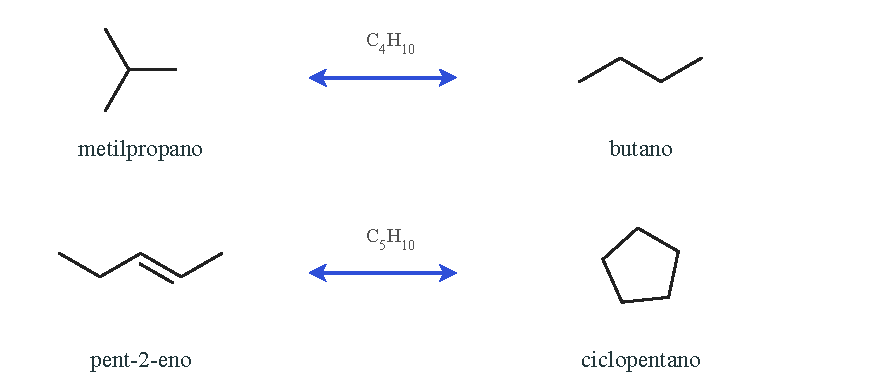
\includegraphics[width=0.70\linewidth]{FigurasSVG/UD9_Quimica_Organica/pdf/UD9_01_isomeria_cadena.pdf}
        \caption{Isomería de cadena}
    \end{figure}

    \item \negsubro{Isomería de posición}. Los compuestos presentan el \textbf{mismo grupo funcional}, pero la posición en la que se encuentra es distinta.

    \begin{figure}[H]
        \centering
        % [FIGURA ORIGINAL] \includegraphics[scale=1]{images/imagesUD9Organica/UD9_Teoria/isomeria_posicion.eps}
        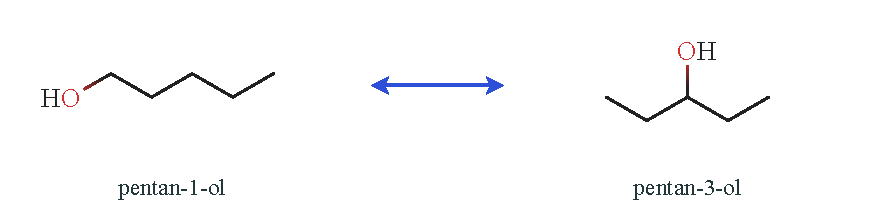
\includegraphics[width=0.70\linewidth]{FigurasSVG/UD9_Quimica_Organica/pdf/UD9_02_isomeria_posicion.pdf}
        \caption{Isomería de posición.}
    \end{figure}

    \item \negsubro{Isomería de función}. Son compuestos que tienen un grupo funcional diferente.

    \begin{figure}[H]
        \centering
        % [FIGURA ORIGINAL] \includegraphics[scale=1]{images/imagesUD9Organica/UD9_Teoria/isomeria_funcion_a.eps}
        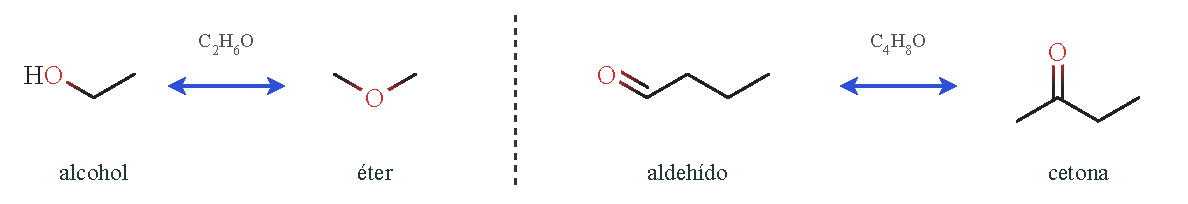
\includegraphics[width=0.95\linewidth]{FigurasSVG/UD9_Quimica_Organica/pdf/UD9_03_isomeria_funcion_a.pdf}
        \caption{Isomería de función. Alcoholes-éteres y aldehídos-cetonas}
    \end{figure}

    \begin{figure}[H]
        \centering
        % [FIGURA ORIGINAL] \includegraphics[scale=1]{images/imagesUD9Organica/UD9_Teoria/isomeria_funcion_b.eps}
        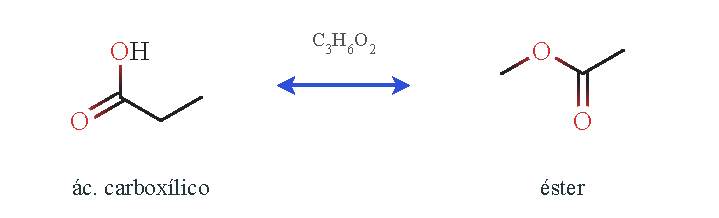
\includegraphics[width=0.57\linewidth]{FigurasSVG/UD9_Quimica_Organica/pdf/UD9_04_isomeria_funcion_b.pdf}
        \caption{Isomería de función. Ácidos carboxílicos-ésteres.}
    \end{figure}

    % \begin{figure}[H]
    %     \centering
    %     \includegraphics[scale=1]{UD9_Teoria/isomeria_funcion.eps}
    % \end{figure}

    Cuando nos pidan un isómero de función de un determinado grupo funcional los podemos asociar de la siguiente manera:

    \begin{enumerate}
        \item Alcoholes \(\iff\) éteres.
        \item Aldehídos \(\iff\) cetonas.
        \item Ácidos carboxílicos \(\iff\) ésteres.
    \end{enumerate}
\end{enumerate}

\subsubsection{Isomería espacial}

\begin{enumerate}[label=\numberballmDarkTeal]
    \item \negsubro{Isomería geométrica}.

    Esta isomería se produce en moléculas rígidas que tengan carbonos con hibridación \(sp^2\) (un alqueno, por ejemplo). Para ello debemos determinar los sustituyentes que están unidos tanto a la izquierda como a la derecha del doble enlace y ver su orientación.

    Antes de ver los tipos de isomería geométrica tenemos que determinar o dar prioridad a los grupos unidos a ese doble enlace. Para asignar la prioridad de los grupos seguiremos la regla de Cahn-Ingold-Prelog (CIP).

    \begin{itemize}
        \item La prioridad se establece según el número atómico del átomo sustituyente, es decir, el átomo unido al doble enlace. Un átomo tiene prioridad sobre otros de número atómico menor. Así pues, el hidrógeno es el que tiene una prioridad más baja.
        % En caso de isótopos, el de mayor masa atómica tiene prioridad.
        \item Si entre dos o más sustituyentes existe coincidencia en el número atómico del átomo unido directamente a la posición cuya prioridad se quiere establecer, se avanza a lo largo de la cadena de cada sustituyente hasta poder asignar un orden de prioridades.
        \begin{figure}[H]
            \centering
            % [FIGURA ORIGINAL] \includegraphics[scale=1]{images/imagesUD9Organica/UD9_Teoria/CIP.eps}
            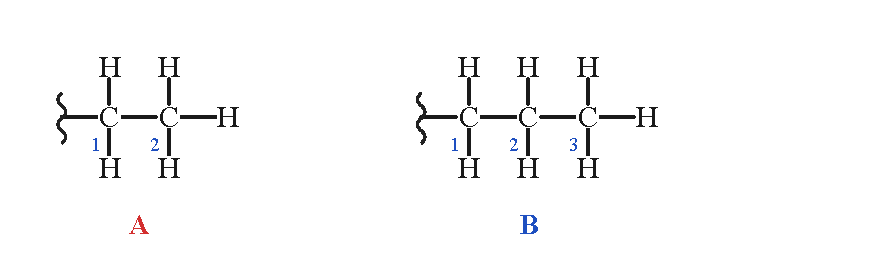
\includegraphics[width=0.70\linewidth]{FigurasSVG/UD9_Quimica_Organica/pdf/UD9_05_reglas_CIP.pdf}
        \end{figure}
    \end{itemize}

    En la siguiente imagen tenemos dos moléculas A y B como sustituyentes. La línea vertical ondulada nos indica donde se encuentra unido al doble enlace. Primero nos fijamos en el primer átomo de carbono (átomo 1) unido al doble enlace: en este caso, en las dos moléculas el átomo unido es el carbono y, por tanto, no podemos asignar una prioridad. Ahora nos centramos en ese átomo de carbono y vemos qué átomos tiene unidos; en ambos casos tiene dos hidrógenos y un átomo de carbono (átomo 2), así que tampoco podemos asignar una prioridad. Ahora nos fijamos en ese átomo 2 de carbono y vemos que el de la molécula A tiene unidos tres átomos de hidrógeno, mientras que el de la molécula B tiene dos átomos de hidrógeno y un átomo de carbono. En este caso sí hay una diferencia y, como la molécula B tiene un átomo con mayor número atómico, la molécula B tendrá prioridad.

    Si tenemos un doble enlace, se considerará ese doble enlace como dos enlaces \ch{C-C}, mientras que si tenemos un grupo carbonilo (\ch{C=O}) se considerará como dos enlaces \ch{C-O}.

    Tenemos dos tipos de isomería:

    \begin{enumerate}[label=\numberballmDarkTeal]
        \item \negsubro{Z o \textit{cis-}}: es aquella en la que los grupos prioritarios se encuentran en el mismo lado.
        \item  \negsubro{E o \textit{trans-}}: es aquella en la que los grupos prioritarios se encuentran en lados opuestos.
        \begin{figure}[H]
            \centering
            % [FIGURA ORIGINAL] \includegraphics[scale=1]{images/imagesUD9Organica/UD9_Teoria/cis_trans.eps}
            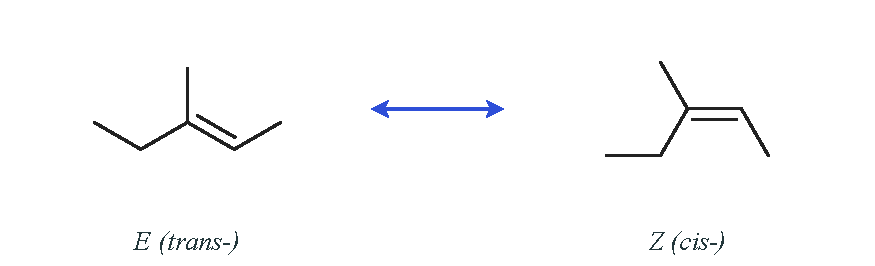
\includegraphics[width=0.70\linewidth]{FigurasSVG/UD9_Quimica_Organica/pdf/UD9_06_isomeria_cis_trans.pdf}
            \caption{Isomería Z/E (cis/trans)}
        \end{figure}
    \end{enumerate}

    Hoy en día, la nomenclatura \textit{cis-} / \textit{trans-} se usa más cuando esos grupos prioritarios son los mismos.

    \item \negsubro{Estereoisomería}. Este tipo de isomería espacial se da en compuestos que tengan un carbono \textbf{estereogénico} o centro \textbf{quiral}, que es aquel que tiene sus 4 sustituyentes diferentes. Estos compuestos se dicen que son compuestos \textbf{quirales}.

    \begin{figure}[H]
        \centering
        % [FIGURA ORIGINAL] \includegraphics[scale=1]{images/imagesUD9Organica/UD9_Teoria/quiralidad.eps}
        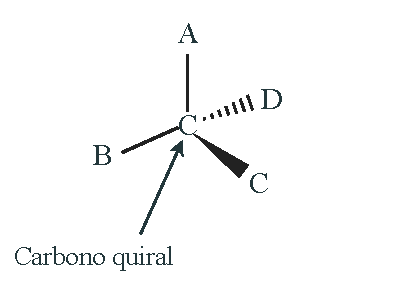
\includegraphics[width=0.33\linewidth]{FigurasSVG/UD9_Quimica_Organica/pdf/UD9_07_carbono_quiral.pdf}
        \caption{Carbono quiral.}
    \end{figure}

    En esta figura, tenemos un compuesto con un carbono quiral, siendo A, B, C y D cuatro sustituyentes distintos entre sí.

    Cuando tenemos un centro quiral, podemos tener dos isómeros llamados \textbf{estereoisómeros} que son el isómero \rectus{} (rectus) y el isómero \sinister{} (sinister). Para determinar si tenemos el isómero \rectus{} o el isómero \sinister{} debemos seguir las siguientes reglas:

    \begin{itemize}
        \item Primero asignamos la prioridad de cada átomo siguiendo las reglas CIP vistas anteriormente.
        \item El de menor prioridad lo situamos lo más alejado de nosotros, es decir, lo ponemos hacia dentro del plano (normalmente es el hidrógeno).
        \item Numeramos los sustituyentes según su prioridad. Al de mayor prioridad le pondremos el 1, al siguiente el 2 y el 3 será el que tenga menor prioridad, sin contar el grupo que hemos situado hacia dentro del plano.
        \item Luego unimos el grupo 1 y el grupo 3 pasando por el grupo 2. Si la dirección descrita sigue el sentido de las agujas del reloj, diremos que tenemos el isómero \rectus{}, mientras que si la dirección sigue el sentido contrario a las agujas del reloj, diremos que es el \sinister{}.
    \end{itemize}

    \begin{figure}[H]
        \centering
        % [FIGURA ORIGINAL] \includegraphics[scale=1]{images/imagesUD9Organica/UD9_Teoria/R_S.eps}
        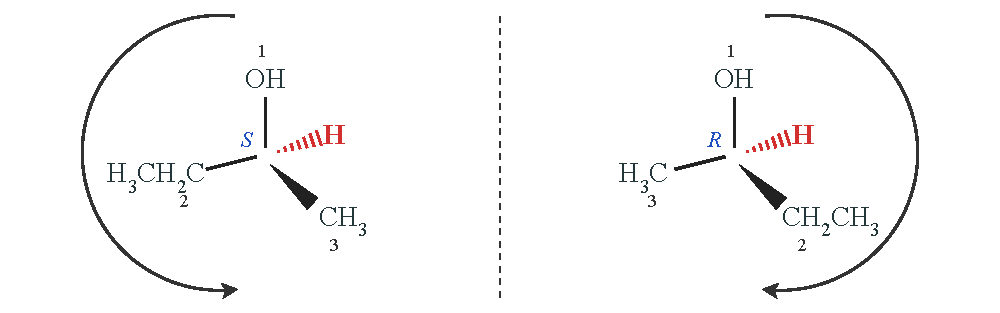
\includegraphics[width=0.80\linewidth]{FigurasSVG/UD9_Quimica_Organica/pdf/UD9_08_configuracion_R_S.pdf}
        \caption{Obtención de la configuración \rectus y \sinister}
    \end{figure}

    Los isómeros \rectus y \sinister diremos que son \textbf{enantiómeros} y son imágenes especulares, es decir, no son superponibles.

    \begin{figure}[H]
        \centering
        % [FIGURA ORIGINAL] \includegraphics[scale=0.5]{images/imagesUD9Organica/UD9_Teoria/imagen_especular.png}
        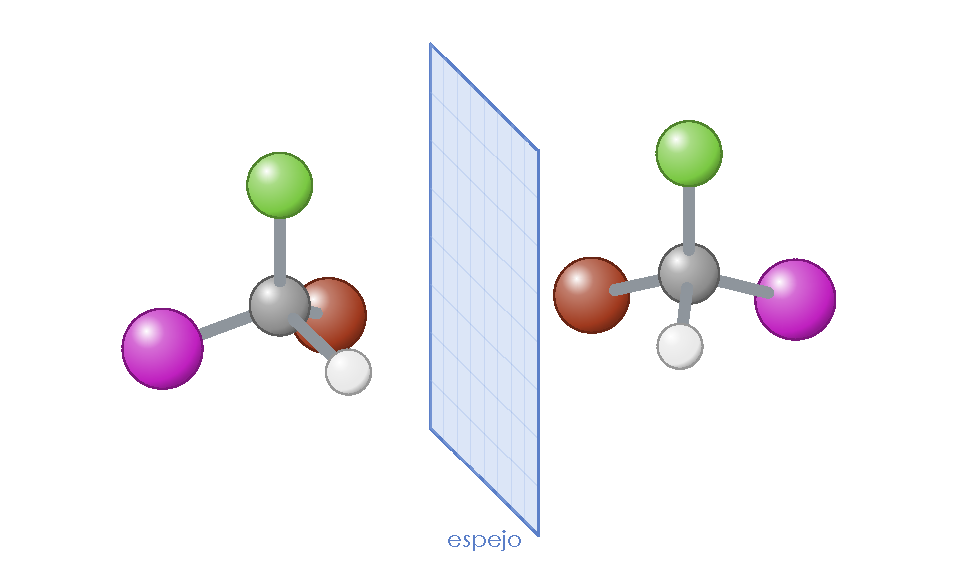
\includegraphics[width=0.6\linewidth]{FigurasSVG/UD9_Quimica_Organica/pdf/UD9_09_imagen_especular.pdf}
        \caption{Imágenes especulares de un compuesto.}
    \end{figure}
\end{enumerate}


\section{Reactividad de los compuestos orgánicos}

En una reacción orgánica, necesitaremos uno o varios compuestos orgánicos, así como una serie de reactivos que ayudarán a que se produzca esa reacción química para formar el producto deseado. Como en toda reacción química, se debe producir primero la ruptura de una serie de enlaces y posteriormente la formación de unos nuevos enlaces.

% \marcador{Breve introducción}

\subsection{Tipos de ruptura de los enlaces}

Tenemos dos tipos de ruptura:

\begin{enumerate}[label=\numberballmDarkTeal]
    \item \negsubro{Ruptura homolítica}: cada átomo que forma el enlace se lleva un electrón (el electrón que había compartido) formando dos radicales. Un radical es una especie que tiene un electrón solitario.
    \begin{figure}[H]
        \centering
        % [FIGURA ORIGINAL] \includegraphics[scale=1]{images/imagesUD9Organica/UD9_Teoria/homolitica.eps}
        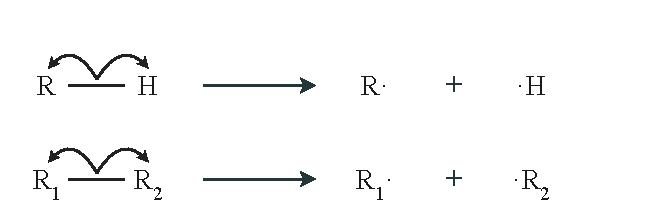
\includegraphics[width=0.53\linewidth]{FigurasSVG/UD9_Quimica_Organica/pdf/UD9_10_ruptura_homolitica.pdf}
    \end{figure}
    \item \negsubro{Ruptura heterolítica}: en este caso, el átomo más electronegativo se lleva los dos electrones del enlace, formando así un anión y un catión. Cuando el catión formado es un compuesto orgánico se llama \textbf{carbocatión}, y si es un anión, \textbf{carbanión}.
    \begin{figure}[H]
        \centering
        % [FIGURA ORIGINAL] \includegraphics[scale=1]{images/imagesUD9Organica/UD9_Teoria/heterolitica.eps}
        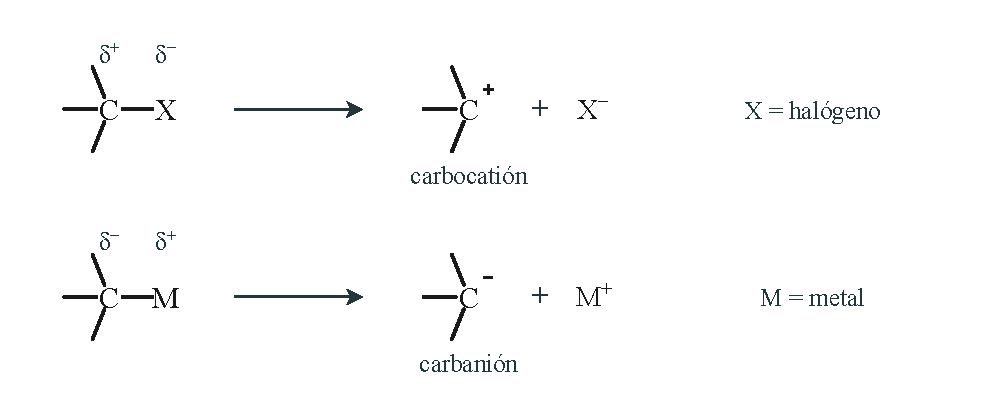
\includegraphics[width=0.80\linewidth]{FigurasSVG/UD9_Quimica_Organica/pdf/UD9_11_ruptura_heterolitica.pdf}
    \end{figure}
\end{enumerate}

\subsection{Tipos de reactivos: nucleófilos y electrófilos}

Tenemos dos tipos de reactivos principalmente:

\begin{enumerate}[label=\numberballmDarkTeal]
    \item \negsubro{Nucleófilos} (\ch{Nu-}). Son aquellos que contienen átomos que pueden ceder electrones y, por tanto, suelen tener carga negativa.

    \item \negsubro{Electrófilos} (\ch{E+}). Son aquellos que contienen átomos que pueden captar electrones.
\end{enumerate}


\begin{table}[H]
    \centering
    \caption{Ejemplos de nucleófilos y electrófilos}
    \vspace{-5pt}
    % --- tabla antigua ---
    % \begin{tblr}{
        % colspec = {| Q[c,m] | Q[c,m] | },
        % row{odd} = {bg=myOrange3!10},
        % row{1} = {bg=myOrange3!90,fg=white,font=\bfseries}
    % }
        % \hline
        % Reactivos nucleófilos & Reactivos electrófilos \\
        % \hline
        % \ch{H2O} & \ch{H3O+} \\
        % \ch{NH3} & \ch{R-CHO} \\
        % \ch{R-OH} & \ch{BF3} \\
        % \ch{R-NH2} & \ch{R_1-CO-R_2} \\
        % \ch{X-} & \ch{X2} (X = halógeno) \\
        % \ch{CN-} &  \\
        % \ch{OH-} &  \\
        % \ch{RO-} &  \\
        % \ch{R-COO-} &  \\
        % \hline
    % \end{tblr}
    % --- tabla nueva ---
    \begin{tabular}{@{}cc@{}}
        \toprule
        \textbf{Reactivos nucleófilos} & \textbf{Reactivos electrófilos} \\
        \midrule
        \ch{H2O} & \ch{H3O+} \\[3pt]
        \ch{NH3} & \ch{R-CHO} \\[3pt]
        \ch{R-OH} & \ch{BF3} \\[3pt]
        \ch{R-NH2} & \ch{R_1-CO-R_2} \\[3pt]
        \ch{X-} & \ch{X2} (X = halógeno) \\[3pt]
        \ch{CN-} &  \\[3pt]
        \ch{OH-} &  \\[3pt]
        \ch{RO-} &  \\[3pt]
        \ch{R-COO-} &  \\
        \bottomrule
    \end{tabular}
\end{table}


\section{Tipos de reacciones orgánicas}

\begin{enumerate}[label=\numberballmDarkTeal]
    \item \negsubro{Reacciones de sustitución}: Son reacciones en las que se sustituye un elemento por otro.
    \begin{figure}[H]
        \centering
        % [FIGURA ORIGINAL] \includegraphics[scale=1]{images/imagesUD9Organica/UD9_Teoria/sustitucion_general.eps}
        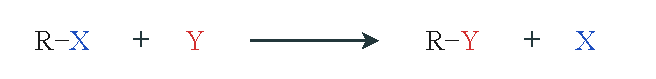
\includegraphics[width=0.53\linewidth]{FigurasSVG/UD9_Quimica_Organica/pdf/UD9_12_sustitucion_general.pdf}
    \end{figure}
    \begin{itemize}
        \item \negsubro{Sustitución radicalaria}: se produce una ruptura homolítica de los enlaces por acción de la luz (se representa por \(h\nu\)). Un ejemplo característico es la halogenación de alcanos, es decir la sustitución de un átomo de H por un halógeno.

        \begin{centeredequation}
            \ch{CH4 + Cl2 ->[\(h\nu\)] CH3Cl + HCl}
        \end{centeredequation}
        \item \negsubro{Sustitución nucleofílica}: se produce cuando un reactivo nucleófilo ataca a un carbono electrófilo. En la mayoría de las ocasiones no tendremos un carbono con la carga positiva, pero sí podemos intuir que el carbocatión se irá formando durante la reacción. Por norma general cuando existe un halógeno unido a un carbono, este se llevará los electrones produciendo una ruptura heterolítica formando así el carbocatión necesario.
        \begin{figure}[H]
            \centering
            % [FIGURA ORIGINAL] \includegraphics[scale=1]{images/imagesUD9Organica/UD9_Teoria/sustitucion_nucleofilica_general.eps}
            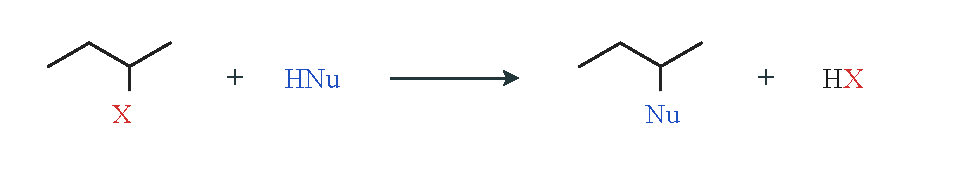
\includegraphics[width=0.77\linewidth]{FigurasSVG/UD9_Quimica_Organica/pdf/UD9_13_sustitucion_nucleofila.pdf}
        \end{figure}
        \begin{itemize}
            \item Sustitución de un halógeno por otro:
            \begin{figure}[H]
                \centering
                % [FIGURA ORIGINAL] \includegraphics[scale=1]{images/imagesUD9Organica/UD9_Teoria/sustitucion_halogeno.eps}
                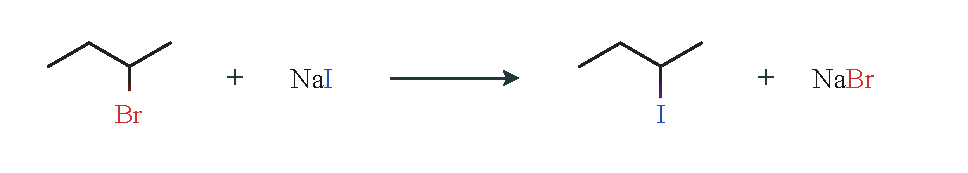
\includegraphics[width=0.77\linewidth]{FigurasSVG/UD9_Quimica_Organica/pdf/UD9_14_sustitucion_halogeno.pdf}
            \end{figure}
            \item Transformación de un derivado halogenado en un alcohol:
            \begin{figure}[H]
                \centering
                % [FIGURA ORIGINAL] \includegraphics[scale=1]{images/imagesUD9Organica/UD9_Teoria/halogeno_y_alcohol.eps}
                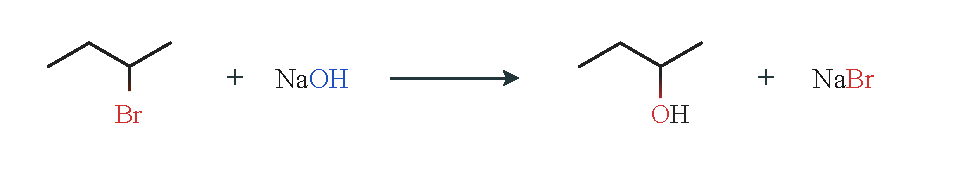
\includegraphics[width=0.77\linewidth]{FigurasSVG/UD9_Quimica_Organica/pdf/UD9_15_halogenuro_a_alcohol.pdf}
            \end{figure}
            \item Transformación de un derivado halogenado en un éter:
            \begin{figure}[H]
                \centering
                % [FIGURA ORIGINAL] \includegraphics[scale=1]{images/imagesUD9Organica/UD9_Teoria/halogeno_y_alcohol_2.eps}
                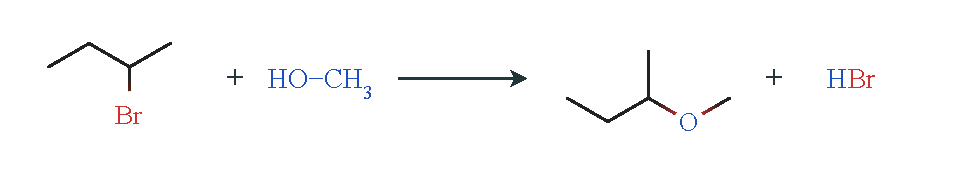
\includegraphics[width=0.77\linewidth]{FigurasSVG/UD9_Quimica_Organica/pdf/UD9_16_halogenuro_a_eter.pdf}
            \end{figure}
            \item Transformación de un derivado halogenado en una amina primaria:
            \begin{figure}[H]
                \centering
                % [FIGURA ORIGINAL] \includegraphics[scale=1]{images/imagesUD9Organica/UD9_Teoria/halogeno_y_amina.eps}
                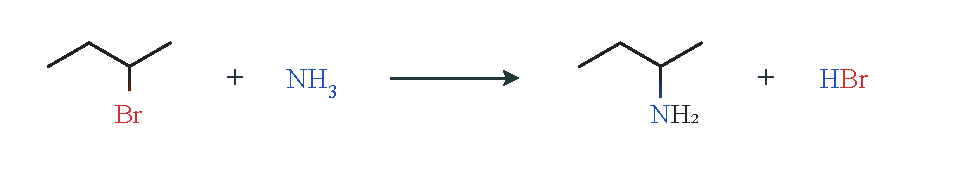
\includegraphics[width=0.77\linewidth]{FigurasSVG/UD9_Quimica_Organica/pdf/UD9_17_halogenuro_a_amina.pdf}
            \end{figure}
            \item Transformación de un derivado halogenado en una amina secundaria o terciaria:

        \end{itemize}
    \end{itemize}

    \item \negsubro{Reacciones de eliminación}: en este tipo de reacciones, se producirá la eliminación de dos átomos formando posteriormente un doble (lo más común) o un triple enlace. En este tipo de reacciones normalmente se requiere una \textbf{base}, a excepción de la deshidratación de alcoholes, que requiere un \textbf{ácido}.
    \begin{figure}[H]
        \centering
        % [FIGURA ORIGINAL] \includegraphics[scale=1]{images/imagesUD9Organica/UD9_Teoria/eliminacion_general.eps}
        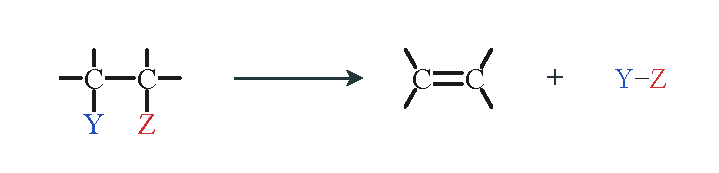
\includegraphics[width=0.57\linewidth]{FigurasSVG/UD9_Quimica_Organica/pdf/UD9_18_eliminacion_general.pdf}
    \end{figure}
    \begin{itemize}
        \item Deshidratación de alcoholes.
        \begin{figure}[H]
            \centering
            % [FIGURA ORIGINAL] \includegraphics[scale=1]{images/imagesUD9Organica/UD9_Teoria/deshidratacion_alcoholes.eps}
            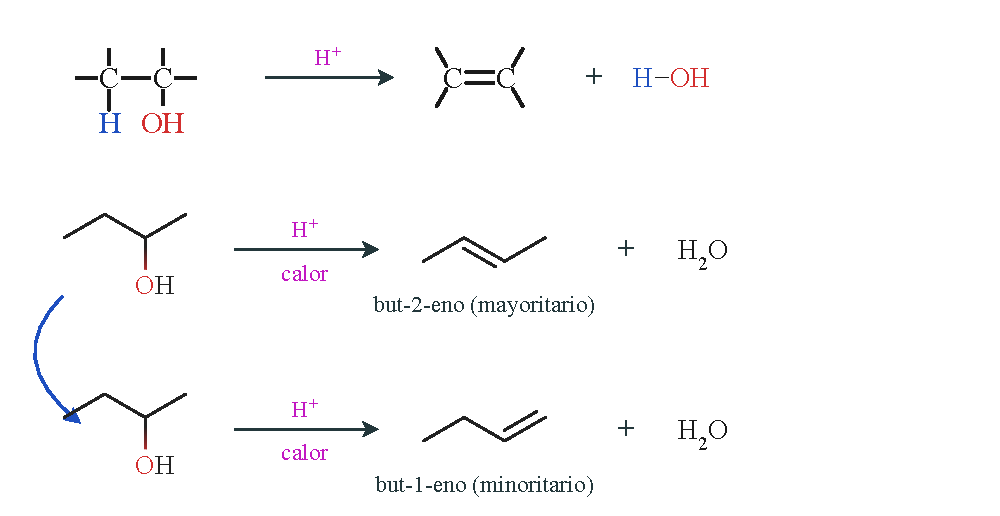
\includegraphics[width=0.80\linewidth]{FigurasSVG/UD9_Quimica_Organica/pdf/UD9_19_deshidratacion_alcoholes.pdf}
        \end{figure}
        \item Deshidrohalogenación de derivados halogenados. X representa el halógeno
        %   \begin{figure}[H]
        %       \centering
        %       \includegraphics[scale=1]{UD9_Teoria/deshalogenacion.eps}
        %   \end{figure}
        \begin{figure}[H]
            \centering
            % [FIGURA ORIGINAL] \includegraphics[scale=1]{images/imagesUD9Organica/UD9_Teoria/deshalogenacion_a.eps}
            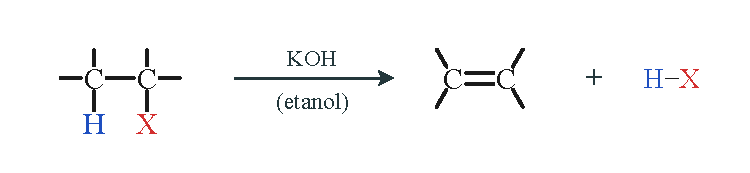
\includegraphics[width=0.60\linewidth]{FigurasSVG/UD9_Quimica_Organica/pdf/UD9_20_deshidrohalogenacion_general.pdf}
        \end{figure}
        \begin{figure}[H]
            \centering
            % [FIGURA ORIGINAL] \includegraphics[scale=1]{images/imagesUD9Organica/UD9_Teoria/deshalogenacion_b.eps}
            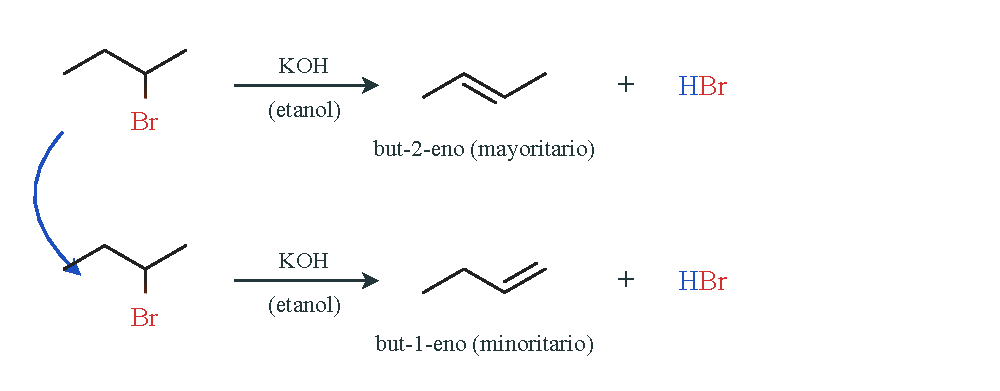
\includegraphics[width=0.80\linewidth]{FigurasSVG/UD9_Quimica_Organica/pdf/UD9_21_deshidrohalogenacion_ejemplo.pdf}
        \end{figure}
    \end{itemize}

        {\normalfont\large\sffamily\bfseries\color{darkblue!80} Formación de alquenos asimétricos}

    Un alqueno asimétrico es aquel que tiene sustituyentes diferentes a ambos lados del doble enlace. Para este tipo de reacciones se sigue la regla de \textbf{Saytzev} que dice que siempre se formará el alqueno más sustituido (por ser más estable). El alqueno más sustituido será aquel que tenga más sustituyentes diferentes al hidrógeno unidos a los carbonos que forman el doble enlace.

    \begin{figure}[H]
        \centering
        % [FIGURA ORIGINAL] \includegraphics[scale=1]{images/imagesUD9Organica/UD9_Teoria/saytzev.eps}
        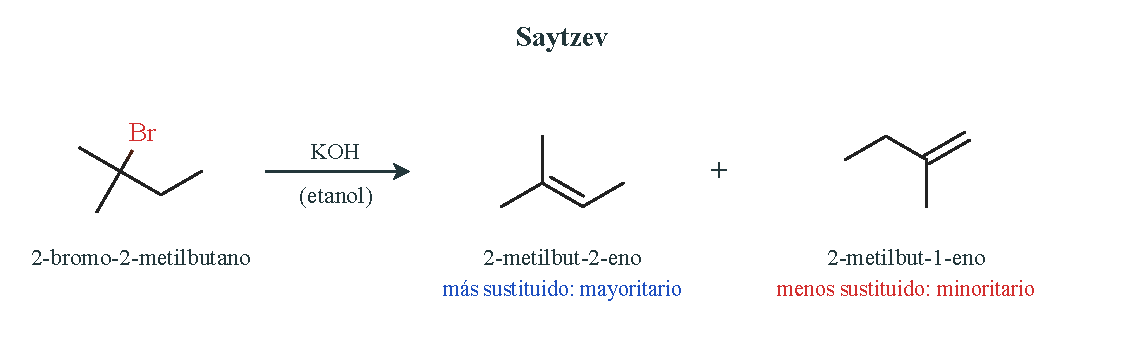
\includegraphics[width=0.90\linewidth]{FigurasSVG/UD9_Quimica_Organica/pdf/UD9_22_regla_saytzev.pdf}
    \end{figure}

    \item \negsubro{Reacciones de adición}: es la adición de un reactivo a un doble o triple enlace.
    \begin{figure}[H]
        \centering
        % [FIGURA ORIGINAL] \includegraphics[scale=1]{images/imagesUD9Organica/UD9_Teoria/adicion_general.eps}
        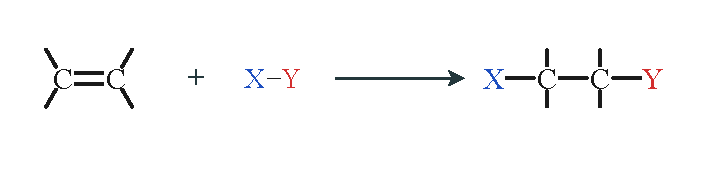
\includegraphics[width=0.57\linewidth]{FigurasSVG/UD9_Quimica_Organica/pdf/UD9_23_adicion_general.pdf}
    \end{figure}
    \begin{itemize}
        \item Hidrogenación de alquenos (adición de \ch{H2}) para dar alcanos:
        \begin{figure}[H]
            \centering
            % [FIGURA ORIGINAL] \includegraphics[scale=1]{images/imagesUD9Organica/UD9_Teoria/adicion_de_hidrogeno.eps}
            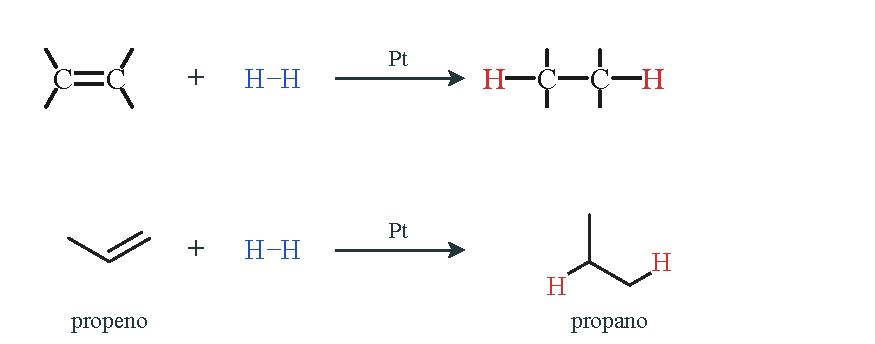
\includegraphics[width=0.70\linewidth]{FigurasSVG/UD9_Quimica_Organica/pdf/UD9_24_adicion_hidrogeno.pdf}
        \end{figure}
        \item Hidratación (adición de \ch{H2O}) de alquenos para dar alcoholes:
        \begin{figure}[H]
            \centering
            % [FIGURA ORIGINAL] \includegraphics[scale=1]{images/imagesUD9Organica/UD9_Teoria/adicion_de_agua.eps}
            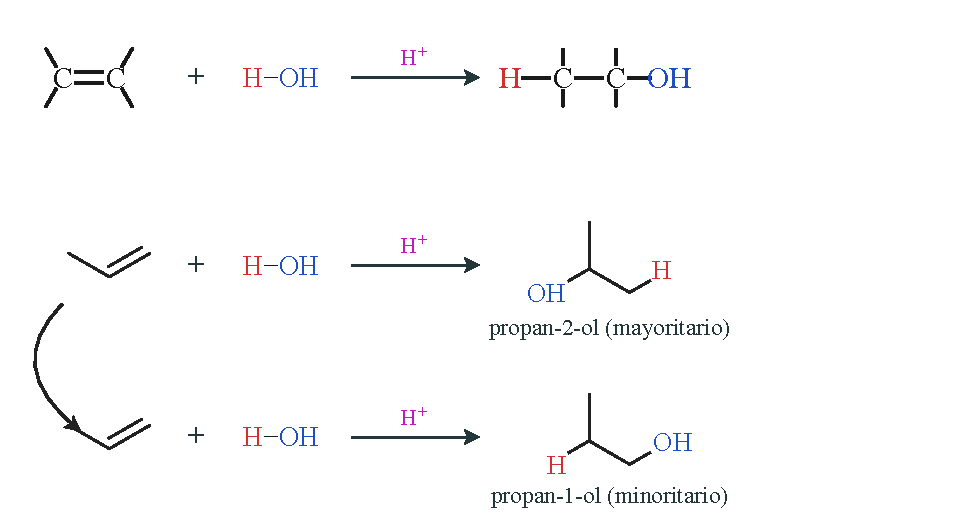
\includegraphics[width=0.77\linewidth]{FigurasSVG/UD9_Quimica_Organica/pdf/UD9_25_adicion_agua.pdf}
        \end{figure}
        \item Adición de haluros de hidrógeno (\ch{HX}) a alquenos para dar derivados halogenados:
        \begin{figure}[H]
            \centering
            % [FIGURA ORIGINAL] \includegraphics[scale=1]{images/imagesUD9Organica/UD9_Teoria/adicion_haluros_hidrogeno.eps}
            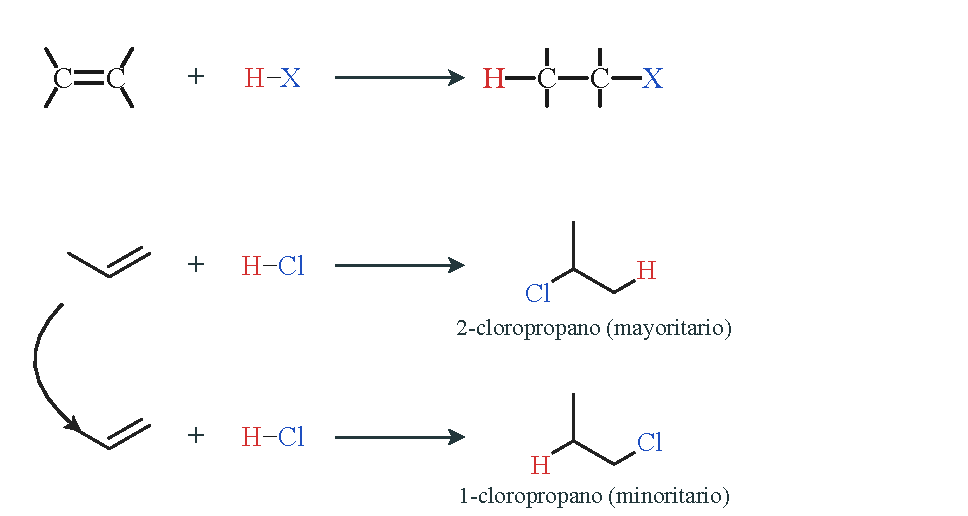
\includegraphics[width=0.77\linewidth]{FigurasSVG/UD9_Quimica_Organica/pdf/UD9_26_adicion_haluros_hidrogeno.pdf}
        \end{figure}
        \item Adición de halógenos (\ch{X2}) a alquenos para dar dihalógenos vecinales:
        \begin{figure}[H]
            \centering
            % [FIGURA ORIGINAL] \includegraphics[scale=1]{images/imagesUD9Organica/UD9_Teoria/adicion_halogenos.eps}
            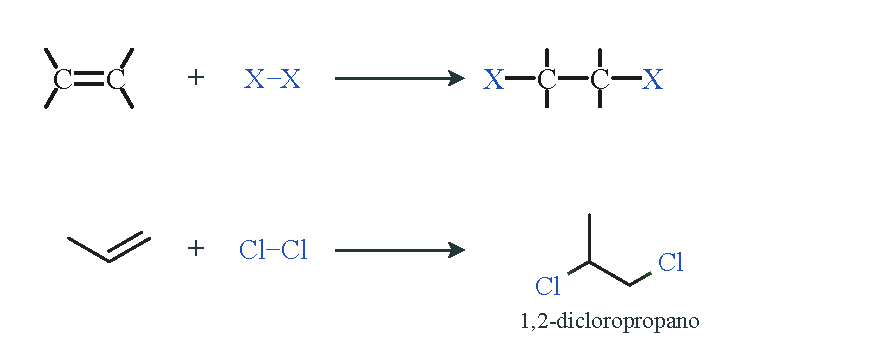
\includegraphics[width=0.70\linewidth]{FigurasSVG/UD9_Quimica_Organica/pdf/UD9_27_adicion_halogenos.pdf}
        \end{figure}
    \end{itemize}

        {\normalfont\large\sffamily\bfseries\color{darkblue!80} Adición en alquenos asimétricos}

    Cuando se produce la adición de un compuesto a un alqueno asimétrico (un alqueno que tienen grupos diferentes tanto a la izquierda como a la derecha del doble enlace), el nucleófilo atacará al átomo de carbono más sustituido mientras que el electrófilo será atacado por el carbono menos sustituido. En el caso de la adición de \ch{HCl} el \ch{Cl-} atacará al carbono de la izquierda mientras que el \ch{H+} se unirá al carbono de la derecha.

    \begin{figure}[H]
        \centering
        % [FIGURA ORIGINAL] \includegraphics[scale=1]{images/imagesUD9Organica/UD9_Teoria/markovnikov.eps}
        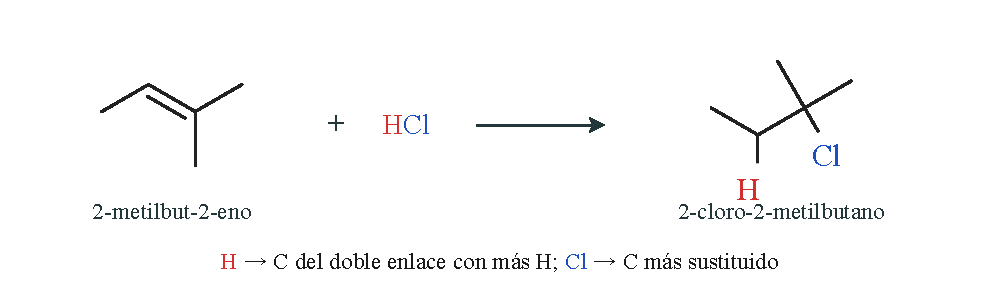
\includegraphics[width=0.80\linewidth]{FigurasSVG/UD9_Quimica_Organica/pdf/UD9_28_regla_markovnikov.pdf}
    \end{figure}

    \item \negsubro{Reacciones de sustitución electrofílica aromática}: son reacciones en las que un electrófilo se ve atacado por un anillo aromático (benceno).
    \begin{figure}[H]
        \centering
        % [FIGURA ORIGINAL] \includegraphics[scale=1]{images/imagesUD9Organica/UD9_Teoria/sustitucion_electrofilica_general.eps}
        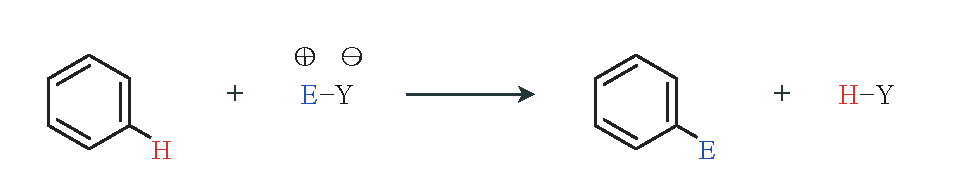
\includegraphics[width=0.77\linewidth]{FigurasSVG/UD9_Quimica_Organica/pdf/UD9_29_sustitucion_electrofila_general.pdf}
    \end{figure}
    Estas reacciones generalmente presentan un catalizador que hace que aumente el carácter electrófilo acelerando así la reacción.
    \begin{itemize}
        \item Halogenación aromática:
        \begin{figure}[H]
            \centering
            % [FIGURA ORIGINAL] \includegraphics[scale=1]{images/imagesUD9Organica/UD9_Teoria/halogenacion_aromatica.eps}
            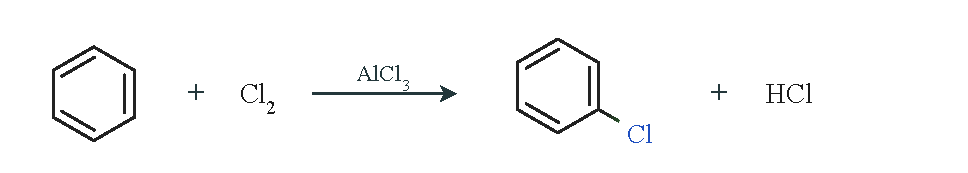
\includegraphics[width=0.77\linewidth]{FigurasSVG/UD9_Quimica_Organica/pdf/UD9_30_halogenacion_aromatica.pdf}
        \end{figure}
        \item Alquilación aromática:
        \begin{figure}[H]
            \centering
            % [FIGURA ORIGINAL] \includegraphics[scale=1]{images/imagesUD9Organica/UD9_Teoria/alquilacion_aromatica.eps}
            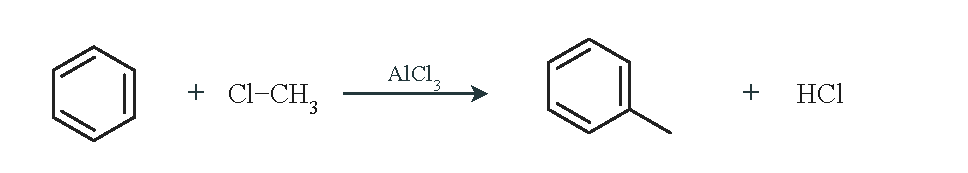
\includegraphics[width=0.77\linewidth]{FigurasSVG/UD9_Quimica_Organica/pdf/UD9_31_alquilacion_aromatica.pdf}
        \end{figure}
        \item Acilación aromática:
        \begin{figure}[H]
            \centering
            % [FIGURA ORIGINAL] \includegraphics[scale=1]{images/imagesUD9Organica/UD9_Teoria/acilacion_aromatica.eps}
            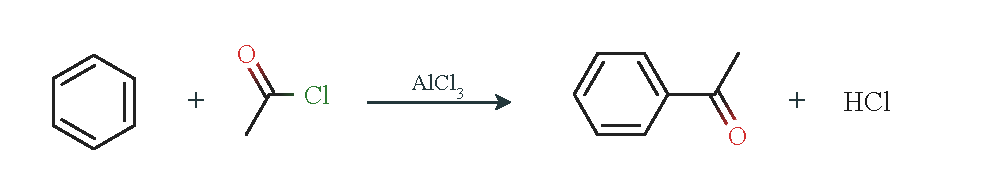
\includegraphics[width=0.80\linewidth]{FigurasSVG/UD9_Quimica_Organica/pdf/UD9_32_acilacion_aromatica.pdf}
        \end{figure}
        \item Nitración aromática:
        \begin{figure}[H]
            \centering
            % [FIGURA ORIGINAL] \includegraphics[scale=1]{images/imagesUD9Organica/UD9_Teoria/nitracion_aromatica.eps}
            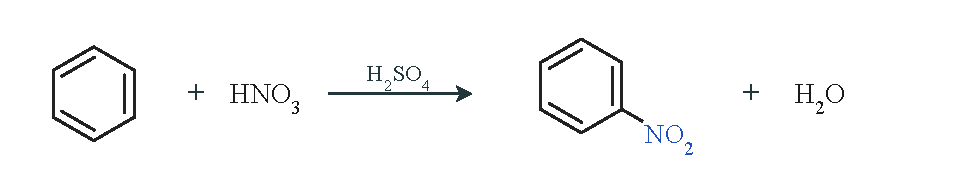
\includegraphics[width=0.77\linewidth]{FigurasSVG/UD9_Quimica_Organica/pdf/UD9_33_nitracion_aromatica.pdf}
        \end{figure}
        \item Sulfonación aromática:
        \begin{figure}[H]
            \centering
            % [FIGURA ORIGINAL] \includegraphics[scale=1]{images/imagesUD9Organica/UD9_Teoria/sulfonacion_aromatica.eps}
            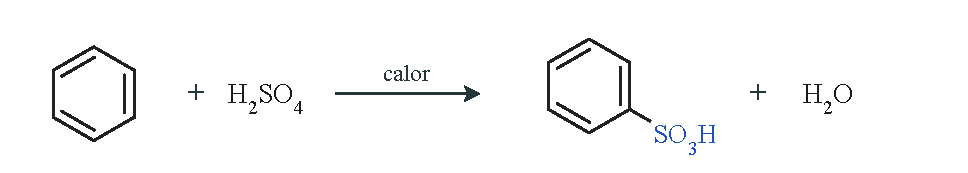
\includegraphics[width=0.77\linewidth]{FigurasSVG/UD9_Quimica_Organica/pdf/UD9_34_sulfonacion_aromatica.pdf}
        \end{figure}
    \end{itemize}
    \item \negsubro{Reacciones de Oxidación-Reducción}: una reacción de oxidación será aquella en la que aumenta el número de átomos de O o disminuye el número de átomos de H. En el caso de la reducción, será cuando aumenta el número de átomos de H o disminuye el número de átomos de O.
    \begin{itemize}
        \item \textbf{Oxidación}: se suelen usar reactivos del tipo \ch{KMnO4}, \ch{K2Cr2O7} o \ch{H2SO4} como oxidantes.

        \item \textbf{Reducción}: se utilizan reactivos del tipo \ch{LiH}, \ch{LiAlH4}, \ch{NaBH4} como reductores.
        \begin{figure}[H]
            \centering
            % [FIGURA ORIGINAL] \includegraphics[scale=1]{images/imagesUD9Organica/UD9_Teoria/oxidacion_reduccion_primarios.eps}
            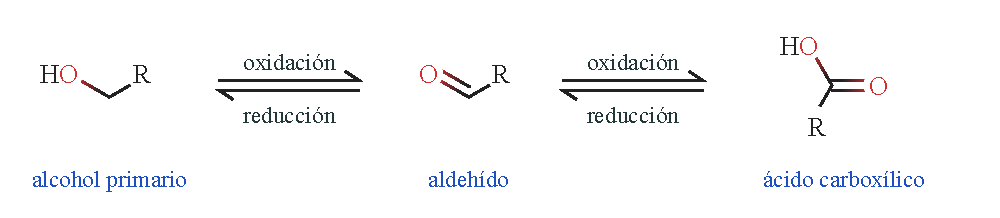
\includegraphics[width=0.80\linewidth]{FigurasSVG/UD9_Quimica_Organica/pdf/UD9_35_oxidacion_alcohol_primario.pdf}
        \end{figure}
        \begin{figure}[H]
            \centering
            % [FIGURA ORIGINAL] \includegraphics[scale=1]{images/imagesUD9Organica/UD9_Teoria/oxidacion_reduccion_secundario.eps}
            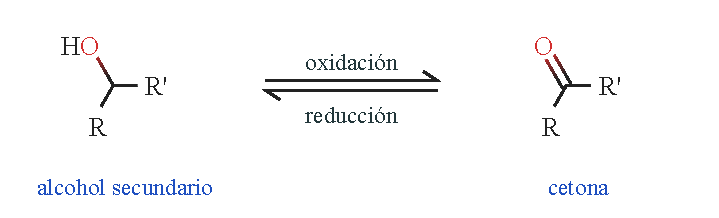
\includegraphics[width=0.57\linewidth]{FigurasSVG/UD9_Quimica_Organica/pdf/UD9_36_oxidacion_alcohol_secundario.pdf}
        \end{figure}
        \begin{figure}[H]
            \centering
            % [FIGURA ORIGINAL] \includegraphics[scale=1]{images/imagesUD9Organica/UD9_Teoria/oxidacion_reduccion_terciario.eps}
            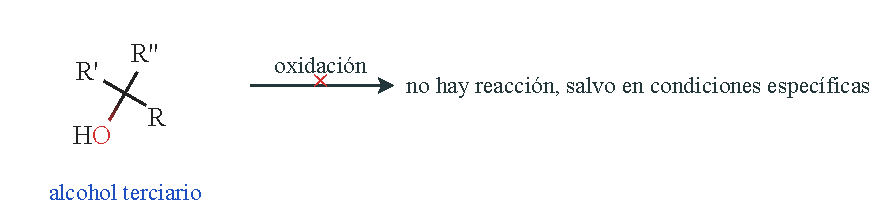
\includegraphics[width=0.70\linewidth]{FigurasSVG/UD9_Quimica_Organica/pdf/UD9_37_oxidacion_alcohol_terciario.pdf}
        \end{figure}
    \end{itemize}
    \item \negsubro{Reacciones de condensación}: son las reacciones en las que dos moléculas orgánicas se unen para formar una molécula de mayor tamaño, perdiéndose una molécula pequeña, generalmente \ch{H2O}.
    \begin{itemize}
        \item Reacción de condensación entre dos moléculas de alcohol para dar un éter.
        \begin{figure}[H]
            \centering
            % [FIGURA ORIGINAL] \includegraphics[scale=1]{images/imagesUD9Organica/UD9_Teoria/condensacion_alcohol_alcohol.eps}
            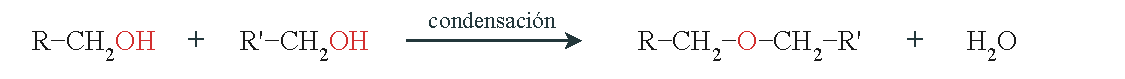
\includegraphics[width=0.90\linewidth]{FigurasSVG/UD9_Quimica_Organica/pdf/UD9_38_condensacion_alcoholes.pdf}
        \end{figure}
        \item Reacción de condensación entre una molécula de ácido carboxílico y un alcohol para formar un éster. A esta reacción se le conoce como \textbf{esterificación}.
        \begin{figure}[H]
            \centering
            % [FIGURA ORIGINAL] \includegraphics[scale=1]{images/imagesUD9Organica/UD9_Teoria/condensacion_acido_alcohol.eps}
            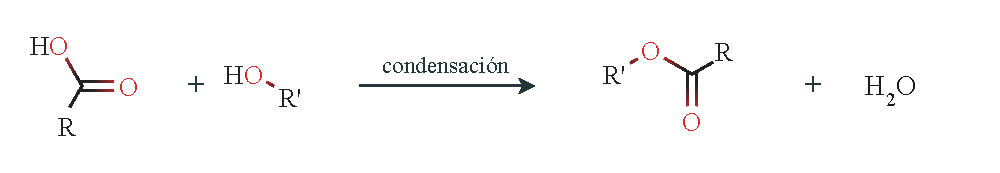
\includegraphics[width=0.80\linewidth]{FigurasSVG/UD9_Quimica_Organica/pdf/UD9_39_condensacion_acido_alcohol.pdf}
        \end{figure}
        \item Reacción entre aminas primarias o secundarias con ácidos carboxílicos para formar amidas.
        \begin{figure}[H]
            \centering
            % [FIGURA ORIGINAL] \includegraphics[scale=1]{images/imagesUD9Organica/UD9_Teoria/condensacion_acido_amina.eps}
            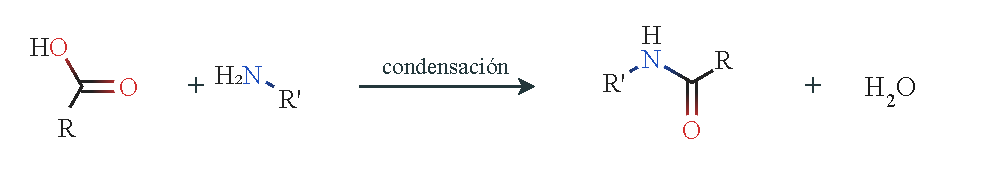
\includegraphics[width=0.80\linewidth]{FigurasSVG/UD9_Quimica_Organica/pdf/UD9_40_condensacion_acido_amina.pdf}
        \end{figure}
    \end{itemize}
    \item \negsubro{Reacciones de hidrólisis}: son reacciones de compuestos orgánicos con agua. Se puede considerar como la reacción opuesta a la reacción de condensación.
    \begin{itemize}
        \item Hidrólisis de éter:
        \begin{figure}[H]
            \centering
            % [FIGURA ORIGINAL] \includegraphics[scale=1]{images/imagesUD9Organica/UD9_Teoria/hidrolisis_eteres.eps}
            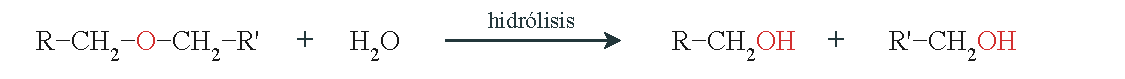
\includegraphics[width=0.90\linewidth]{FigurasSVG/UD9_Quimica_Organica/pdf/UD9_41_hidrolisis_eteres.pdf}
        \end{figure}
        \item Hidrólisis de un éster:
        \begin{figure}[H]
            \centering
            % [FIGURA ORIGINAL] \includegraphics[scale=1]{images/imagesUD9Organica/UD9_Teoria/hidrolisis_ester.eps}
            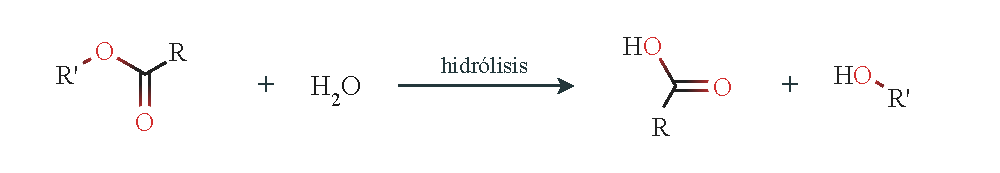
\includegraphics[width=0.80\linewidth]{FigurasSVG/UD9_Quimica_Organica/pdf/UD9_42_hidrolisis_ester.pdf}
        \end{figure}
        \item Hidrólisis de una amida:
        \begin{figure}[H]
            \centering
            % [FIGURA ORIGINAL] \includegraphics[scale=1]{images/imagesUD9Organica/UD9_Teoria/hidrolisis_amida.eps}
            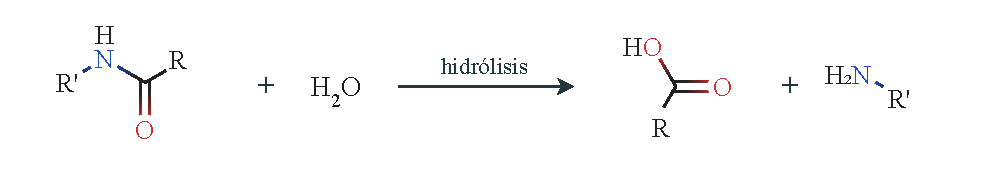
\includegraphics[width=0.80\linewidth]{FigurasSVG/UD9_Quimica_Organica/pdf/UD9_43_hidrolisis_amida.pdf}
        \end{figure}
    \end{itemize}
\end{enumerate}
